\chapter{Models}\label{ch:models}

This chapter presents an exploration of various models used in the automatic generation of 3D models. It bridges the theoretical foundations laid in the previous chapters with practical applications and technologies that are developing the field of 3D modeling. Furthermore, it delves into different categories of model generation, specifically focusing on 3D models generated from text and images. This comprehensive analysis not only highlights the diversity and complexity of current methods but also underscores the rapid advancements and potential future developments in this domain. The below timeline shows the chronological development of these models, offering a perspective on how the field has progressed over time.

\begin{figure}[H]
    \centering
      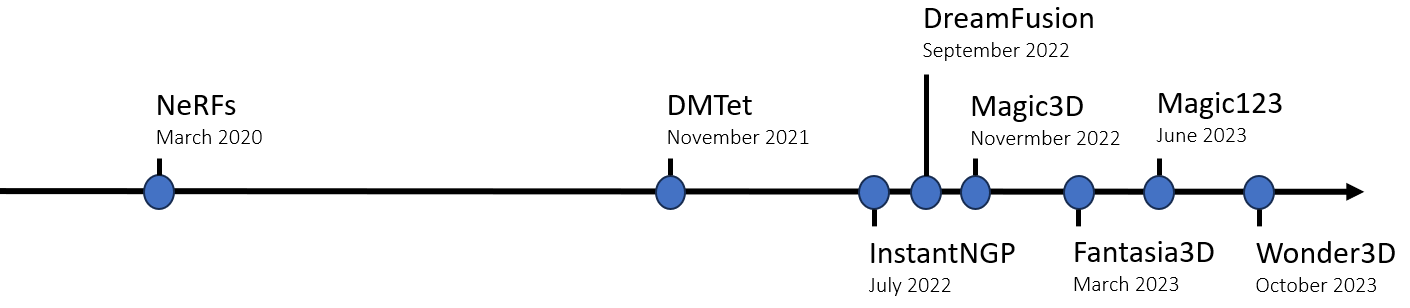
\includegraphics[width=\textwidth]{figures/timelineMethods.png}
      \caption{Timeline of generative 3D modeling technologies: This figure outlines important milestones in the development of the key methods discussed in this thesis.}~\label{fig:timelineMethods}
\end{figure}

The chapter is structured to critically examine the methodologies, strengths, and limitations of each model. This detailed exploration provides an in-depth understanding of the current state of 3D model generation, emphasizing both the technological intricacies and their practical implications.

\section{3D from Text input}\label{3d from text}

In recent years, the field of 3D model generation has witnessed a significant shift, with an increasing focus on generating 3D models from textual descriptions. This innovative approach leverages advancements in natural language processing and deep learning, allowing for the creation of 3D models based purely on textual input. This section delves into the mechanics and applications of such systems, with a specific emphasis on groundbreaking methods like Dreamfusion, Fantasia3D, and Magic 3D.

The ability to generate 3D models from text opens up a plethora of possibilities. For designers, artists, and architects, it translates to a more intuitive and accessible way to bring ideas to life. This technology also holds immense potential in education and entertainment, where it can be used to create interactive and engaging 3D content. In this section, the focus will be on how these systems interpret textual descriptions while explaining the challenges they face, such as ensuring accuracy and maintaining the fidelity of the generated models to the original text.

%\subsection{Dreamfields}
\label{dreamfields}


(The genesis of DreamFusion lies in the evolution of Dream Fields, a generative 3D AI system unveiled by Google in late 2021. Dream Fields initially married OpenAI's image analysis model, CLIP, with Neural Radiance Fields (NeRF) to foster the generation of 3D views from text. DreamFusion further refined this approach by introducing a new loss based on Google's large AI image model, Imagen, thus paving the way for enhanced text to 3D synthesis.)


Dreamfields present a novel approach to generating three-dimensional objects guided by textual input as introduced by \citeauthor{jainDreamFields}. Utilizing a continuous volumetric representation, Dreamfields are capable of producing high-quality, intricate 3D objects that not only adhere to the specified textual descriptions but also exhibit realistic geometry and appearance. This technology leverages pre-trained image and text encoders, providing a zero-shot learning capability that does not require paired text and object data for training \citep{jainDreamFields}.

The methodology in Dreamfields hinges on learning a continuous volumetric representation, termed a Dream Field, for both the geometry and appearance of a 3D object. The aim is to optimize this Dream Field to be consistent with a given textual description, extending the ideas from previous work on visualizing preferred inputs and features of neural networks by optimizing in image space \citep{jainDreamFields}. The Dream Field is modeled as a neural network, \( f: \mathbb{R}^3 \rightarrow \mathbb{R}^4 \), mapping a 3D coordinate \( (x, y, z) \) toa 4D vector \( (r, g, b, \sigma) \) that represents the color and density at that location. The model then employs raymarching to visualize this continuous field, a computational technique that can be understood as moving a camera through the 3D space to capture the object from various angles. Mathematically, this is achieved by integrating the Dream Field along a ray \( R(t) \) emanating from the camera. Essentially, this is like calculating the average color and light intensity the camera "sees" as it looks along this line. The rendered color \( C \) and opacity, or density, \( \alpha \) are computed using the formulas \citep{jainDreamFields}:

\[
C = \int_0^T \alpha(t) \cdot c(t) \cdot \exp\left(-\int_0^t \alpha(s) \, ds\right) \, dt
\]
\[
\alpha = \int_0^T \alpha(t) \cdot \exp\left(-\int_0^t \alpha(s) \, ds\right) \, dt
\]

Here, \( c(t) \) and \( \alpha(t) \) are the color and density at point \( t \) along the ray, \( T \) is the total length of the ray, and \( \exp \) is the exponential function, used to model how light fades or attenuates as it moves through the object. 

The optimization aims to align the rendered image with a given textual description. This phase focuses on minimizing an objective function \( \mathcal{L} \), which essentially quantifies the difference between the generated object and the textual description \citep{jainDreamFields}.

\[
\mathcal{L} = -\frac{E_{\text{img}}(I) \cdot E_{\text{text}}(T)}{\| E_{\text{img}}(I) \| \, \| E_{\text{text}}(T) \|}
\]

Here, \( E_{\text{img}}(I) \) and \( E_{\text{text}}(T) \) are the embeddings of the image and text, respectively, converted into a common numerical language by pre-trained encoders. \( \mathcal{L} \) is minimized when these embeddings are most similar, measured by the cosine of the angle between them (cosine similarity). In summary, Dreamfields integrates these mathematical principles—continuous mapping through neural networks, raymarching for rendering, and optimization based on similarity measures—to fine-tune the geometry and appearance of a 3D object so that it aligns closely with the given textual description \citep{jainDreamFields}.

Dreamfields find applications in numerous domains where 3D object generation is crucial. These include but are not limited to computer-aided design, virtual reality, and augmented reality. Their zero-shot learning capability opens doors for creating complex objects without the need for extensive training data, making them particularly useful in scenarios where paired text-object data are scarce or unavailable \citep{jainDreamFields}.

Dreamfields' approach to generating 3D objects presents a unique blend of advantages and limitations that contribute to its versatility and potential areas for improvement. Among its most notable advantages is the zero-shot learning capability, allowing the model to generate objects based solely on textual descriptions without the need for paired text-object training data. This attribute is particularly advantageous in scenarios where collecting such paired data is either impractical or resource-intensive \citep{jainDreamFields}. Another significant strength lies in its use of a continuous volumetric representation, which enables the creation of intricate and nuanced geometries. Unlike traditional methods that rely on discrete representations like voxel grids, Dreamfields can generate highly detailed and realistic 3D models \citep{jainDreamFields}. Adding to its merits is the unified treatment of both geometry and appearance in a single representation. Traditional approaches often separate these two aspects, which can result in inconsistencies in the final model \citep{jainDreamFields}. Dreamfields elegantly sidestep this issue, producing 3D objects that are both geometrically and aesthetically coherent. Moreover, the model's optimization process offers a high degree of flexibility, capable of adapting to a wide variety of textual inputs. This makes it a versatile tool for generating a diverse range of objects across different domains. However, Dreamfields is not without its limitations. One of the primary challenges is the computational intensity associated with its continuous representation and optimization process \citep{jainDreamFields}. The high computational requirements could constrain its applicability in real-time or resource-limited settings. Another limitation stems from its reliance on pre-trained text and image encoders, which could introduce biases and restrict the diversity of objects that can be generated \citep{jainDreamFields}. The performance of Dreamfields is significantly influenced by the quality of these pre-trained models, which may vary. Furthermore, the model may struggle with textual descriptions that are inherently ambiguous or open to multiple interpretations. While designed to align closely with textual inputs, the current state of Dreamfields may find it challenging to handle overly vague or abstract descriptions effectively \citep{jainDreamFields}.

Dreamfields offer an innovative approach to 3D object generation through textual guidance. By leveraging a continuous volumetric representation and pre-trained encoders, Dreamfields achieve high-quality, detailed, and realistic 3D objects that closely align with the given textual descriptions. While the technology has its limitations, its advantages and potential applications make it a compelling avenue for future research and development in the field of automatic 3D model generation.


\subsection{Dreamfusion}\label{dreamfusion}

DreamFusion, as introduced by \citeauthor{pooleDreamfusion}, marks a significant advancement in the field of 3D modeling. Utilizing Neural Radiance Fields (NeRF), DreamFusion employs a novel technique known as Score Distillation Sampling (SDS) to generate coherent 3D objects and scenes from a variety of text prompts. This approach diverges from traditional methods that depend on pre-existing images from multiple angles, as DreamFusion dynamically generates these images during training using a diffusion model.

Central to DreamFusion is the use of Differentiable Image Parameterization (DIP), as described by \citep{mordvintsevDIP}. This technique enables the generation of images \( x \) through parameters \( \theta \) and a differentiable generator \( g \), offering refined optimization capabilities even at the pixel level \citep{pooleDreamfusion}. This marks a shift from the conventional approach of diffusion models, which usually produce outputs similar to their training data. In DreamFusion, the parameters \( \theta \) define 3D volumes, with \( g \) functioning as a volumetric renderer. 

In the Score Distillation Sampling (SDS) method, the initial step involves identifying the best parameters \( \theta \) for the model. This involves minimizing the loss in relation to a datapoint created by a model.~\citeauthor{pooleDreamfusion} use the formular~\[ \theta^{*} = \text{arg min}_{\theta} \mathcal{L}_{\text{Diff}}(\phi, \mathbf{x} = g(\theta)) \] This essentially means the model is adjusted to find the parameters \( \theta \) that bring its output as close as possible to the desired result based on textual input. The primary SDS function by \citeauthor{pooleDreamfusion} is:~\[
\nabla_{\theta}\mathcal{L}_{\text{SDS}}(\phi,\mathbf{x}=g(\theta))\triangleq\mathbb{E}_{t,\epsilon}\left[w(t)\left(\hat{\epsilon}_{\phi}({\mathbf{z}}_{t};y,t)-\epsilon\right){\frac{\partial\mathbf{x}}{\partial\theta}}\right]
\] In this equation, \( w(t) \) acts as a weighting factor, modifying the influence of different components within the formula. The term \( \hat{\epsilon}_{\phi}({\mathbf{z}}_{t};y,t) \) represents the score function predicted by the diffusion model \( \phi \). This function estimates the noise adjustments needed based on the noisy image \( z_t \), the text embedding \( y \), and the noise level \( t \). The actual noise at time \( t \) is denoted by \( \epsilon \). This function is key in determining how the noise should be adjusted during the diffusion process to align the generated image with the text input. Additionally, the term \( \frac{\partial\mathbf{x}}{\partial\theta} \) indicates how changes in the model’s parameters \( \theta \) affect the image \( \mathbf{x} \), guiding the optimization process. SDS adds controlled noise to an image \( x \) at each timestep \( t \), and then adjusts it based on the model's scoring, efficiently updating the image to closely match the text descriptions without the need for traditional backpropagation \citep{pooleDreamfusion}.

\begin{figure}[ht]
  \centering
    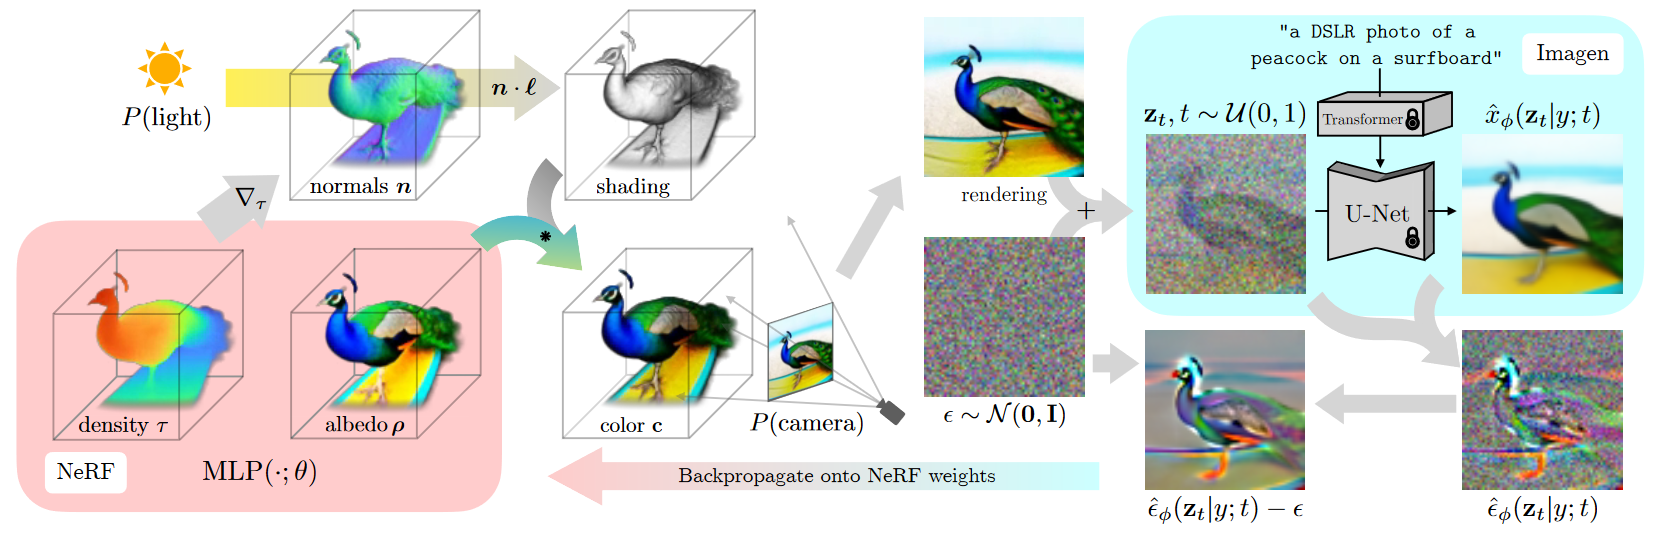
\includegraphics[width=1\columnwidth]{figures/Dreamfusion.png}
    \caption{Summatized functionality of Dreamfusion, image by \citep{pooleDreamfusion}}\label{fig:figureDreamfusion}
  \end{figure}

DreamFusion offers an innovative approach to transforming text into 3D models, as depicted in Figure~\ref{fig:figureDreamfusion}. This process employs several key components: natural language captions for directional guidance, Google's Imagen as the text-to-image diffusion model \citep{saharia2022imagen}, an imporved version of Neural Radiance Field, the mip-NeRF 360 \citep{barron2022mipnerf} ``that reduces aliasing'' \citep{pooleDreamfusion}, and the Score Distillation Sampling (SDS) for the loss function.

At the center of the rendering process is the Neural Radiation Field, which is represented as \( \text{MLP}(\cdot; \theta) \), where the dot \(\cdot\) denotes the input of 3D coordinates and viewing directions. This input is important to determine how light and color interact in 3D space.~\(\theta\) symbolizes the parameters or weights of the MLP that are fine-tuned during training. These parameters determine how the MLP interprets its input (the 3D coordinates and viewing directions) to produce the final output, such as the color and density at each point in the 3D model.

The creation of 3D scenes begins with this parameterization of the NeRF MLP, followed by randomly choosing camera angles and point light positions. This randomness ensures realistic representations from various perspectives. Shading plays a crucial role in adding depth and realism, driven by the interaction of light with surface normals, computed from the density gradients and the light position \( l \). Additionally, the inherent color of objects, or albedo, is generated during the NeRF rendering phase. By combining this albedo with the effects of shading, the NeRF accurately renders the final color for each scene point. The result is a detailed visual representation from the selected viewpoint.

After rendering, DreamFusion evaluates the scene against the diffusion model's predictions, assessing diffusion loss to evaluate the match with the expected outcome. The rendered image is then diffused and reconstructed using a static conditional Imagen model, which adds predicted noise \( \hat{\epsilon}_\phi(z_t | y; t) \) into the rendering, to improve fidelity but also increasing variance \citep{pooleDreamfusion}.

The model refinement phase involves subtracting this predicted noise, resulting in a direction with reduced variance, denoted as \( \text{stopgrad}[\hat{\epsilon}_\phi - \epsilon] \). This direction informs the backpropagation through the rendering process, crucial for updating the NeRF's MLP parameters in a manner that more accurately reflects the scene described by the text. Unlike the SDS method, this backpropagation directly impacts NeRF's rendering pipeline, ensuring parameter adjustments are precisely aligned with the scene's details and nuances.

Despite DreamFusion's promising results, it is not without limitations. The model tends to exhibit a lower level of detail, partly due to its reliance on a \( 64 \times 64 \) image model. Furthermore, while SDS is an effective loss function, it sometimes leads to ``oversaturated and oversmoothed results \([\ldots]\)'' \citep{pooleDreamfusion}. Another aspect to consider with SDS is the mode-seeking behavior, which potentially limits the variety of results generated. This limitation is strengthened by the use of KL divergence, ``which has been previously noted to have mode-seeking properties in the context of variational inference and probability density distilaltion''\citep{pooleDreamfusion}. This tendency of the model to prioritize the most frequent patterns can lead to a trade-off between accuracy and diversity, so ``it may be unclear if minimizing this loss will produce good samples'' \citep{pooleDreamfusion}. This statement highlights a major challenge in machine learning, especially with generative models such as DreamFusion. Minimizing loss, a standard method for improving model performance, does not always lead to high-quality or diverse results. There is a risk of overfitting, where the model can reproduce the training data very well, but is less able to generate new and diverse results.
\subsection{Fantasia3D}\label{fantasia3D}

The model proposed by \citeauthor{chen2023fantasia3d} takes a different approach to generating 3D models from text input, in particular by disentangling geometry and appearance in the generated 3D models.
This method offers a more detailed rendering quality compared to conventional Neural Radiance Fields (NeRFs), which use volume rendering to combine the learning of surface geometry with pixel colors. This conventoional approach limits effective surface recovery, lacking the capability to track the surface of an object and tune detailed material and texture. In contrast, Fantasia3D achieves more realistic outputs with its hybrid scene representation of DMTet, ``which maintains a deformable tetrahedral grid and a differentiable mesh extraction layer; deformation can thus be learned through the layer to explicitly control the shape generation'' \citep{chen2023fantasia3d}

\begin{figure}[ht]
  \centering
    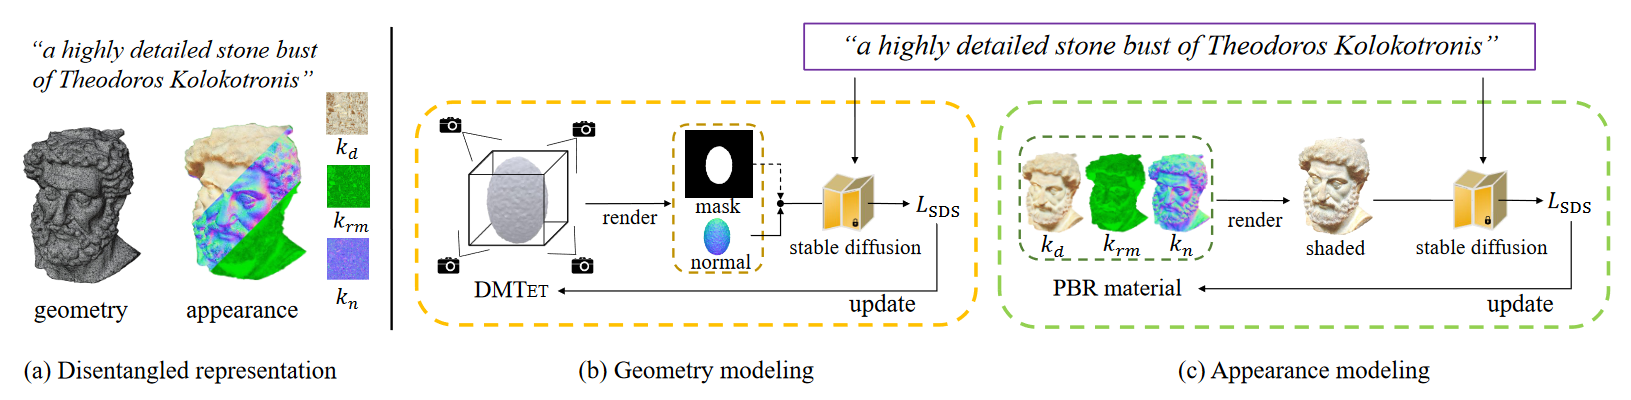
\includegraphics[width=1\columnwidth]{figures/Fantasia3D.png}
    \caption{Overview of Fantasia3D's workflow, disentangling geometry from appearance modeling and iteratively enhancing the quality using a refinment process \citep{chen2023fantasia3d}.}\label{fig:figureFantasia}
\end{figure}

In the geometry stage, Fantasia3D relies on a Deformable Mesh Tetrahedralization (DMTet), which parametrizes the 3D geometry as a Multi-Layer Perceptron (MLP) \(\Psi\). Initially, Fantasia3D renders and encodes surface normals and object masks extracted from DMTet. However, in later stages, the model refines its approach by using only the rendered normal map for shape encoding \citep{chen2023fantasia3d}. The default initialization of DMTet is an ellipsoid, but the model also accepts custom inputs.

Appearance Modeling involves training another MLP \( \Gamma \), which is responsible for applying the Bidirectional Reflectance Distribution Function (BRDF) \citep{chen2023fantasia3d} to a pre-learned DMTet. This function is crucial for ``predict[ing] parameters of surface material and supports high-quality 3D generation via photorealistic rendering'' \citep{chen2023fantasia3d}. The BRDF focuses on the following parameters to achieve accurate shading of the geometry: the diffuse value \(k_d\), the combined roughness and metallic properties \(k_{rm}\), and the normal variation \(k_n\). These are predicted using the formula \((k_d, k_{rm}, k_n) = \Gamma(\beta(p); \gamma)\) by \citeauthor{chen2023fantasia3d}, where \(\beta(p)\) represents the surface properties at point \(p\) and \(\gamma\) denotes network parameters.

Both MLPs (\(\Gamma\) for appearance and \(\Psi\) for geometry) undergo a refinement process, using a pre-trained Stable Diffusion model \citep{rombachStableDiffusion}. This model improves the capabilities of \(\Gamma\) and \(\Psi\), ensuring that they accurately interpret and render 3D shapes and textures. A key aspect of this refinement is the use of Score Distillation Sampling (SDS) loss \citep{mildenhallNERF} for optimization. In this process, SDS loss functions by comparing the true image with the one generated by Fantasia3D. This comparison is achieved through ray casting, where rays are projected for each pixel in the scene. The model then renders the color of each ray, effectively translating the 3D model into a 2D image. This step allows the model to evaluate and adjust its rendering based on how accurately it replicates the true image of Stable Diffusion. By iterating this process, the model continually improves its accuracy in rendering photorealistic images, ensuring that the final output is as close to the actual image as possible.

Fantasia3D offers a high degree of user interactivity, permitting the incorporation of both custom and predefined generic 3D shapes, thus greatly enhancing the versatility and user engagement in the content creation process. The separation of geometry and appearance generation also ensures compatibility with widely-used graphics engines \citep{chen2023fantasia3d}. Despite its capabilities in creating high-quality 3D models from textual descriptions, Fantasia3D encounters specific challenges. One notable limitation is its struggle with accurately generating complex geometries like hair, fur, and grass \citep{chen2023fantasia3d}. Furthermore, the model is currently not able to generate complete scenes as focus is currently lying on individual object generation \citep{chen2023fantasia3d}.

\subsection{Magic3D}\label{magic3D}

Magic3D represents a significant advancement in the domain of high-resolution 3D model generation from text input. Developed by \citeauthor{lin2023magic3d}, this method overcomes limitations observed in previous models like DreamFusion, particularly in terms of optimization speed and resolution of the generated models.

The core technique employed by Magic3D involves a coarse-to-fine optimization process. Initially, a coarse model is generated using a low-resolution diffusion prior, which is then fine-tuned in the second stage to yield a high-quality textured 3D mesh model \citep{lin2023magic3d}. This approach allows Magic3D to generate detailed 3D models with enhanced texture quality in a comparatively shorter time frame.

\begin{figure}[ht]
  \centering
    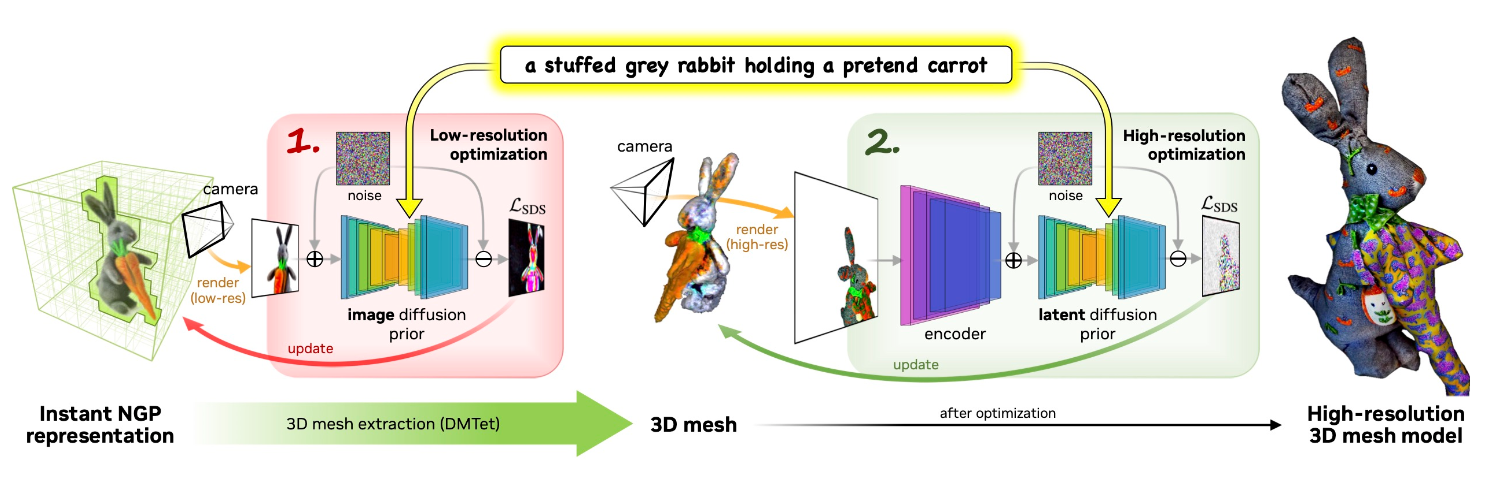
\includegraphics[width=1\columnwidth]{figures/Magic3D.png}
    \caption{This illustration from \citep{lin2023magic3d} showcases the Magic3D process, beginning with the InstantNGP for initial 3D representation. It then details the coarse-to-fine procedure, evolving to a refined high-resolution 3D mesh model.}\label{fig:figureMagic}
\end{figure}


Magic3D's process of generating 3D models from text prompts begins with an initial stage that employs the eDiff-I base diffusion model \citep{balaji2022eDiff-I}, akin to Google's Imagen \citep{saharia2022imagen}. This model operates at a relatively low resolution of \(64 \times 64\), laying the groundwork for the 3D geometry and textures given from the text input \citep{lin2023magic3d}. During this phase, the model uses a sparse 3D hash grid structure from Instant NGP \citep{mueller2022instant}, ``which allows us to represent high-frequency details at a much lower computational cost''~\citep{lin2023magic3d}. The optimization in this phase is performed by two single-layer neural networks that predict albedo (the base color of the object), density (how solid or transparent parts of the object are), and normals (which determine how light bounces off the surface) of the object \citep{lin2023magic3d}. This approach not only speeds up the optimization process but also ensures the foundational quality of the coarse 3D model \citep{lin2023magic3d}. 
This stage involves sampling an image from the NGP representation, which is then infused with an initial state of noise through the image diffusion prior. This step sets the stage for iterative refinement. The refinement is guided by the Score Distillation Sampling (\(L_{SDS}\)) loss function, which evaluates and compares the generated image against a target image, enabling the model to iteratively improve its accuracy. The use of the image diffusion prior in this low-resolution phase is primarily for shaping the overall structure and layout of the model, focusing more on broad features rather than fine details.

In the refinment stage, Magic3D focuses on refining this coarse model into a high-resolution textured mesh, marking a transition from the basic structure to a detailed representation. The refinement process starts with a 3D mesh derived from a deformable tetrahedral grid, where each grid vertex contains a value indicating its distance from the surface (signed distance field) and its deformation from the original position \citep{shen2021DMTet, lin2023magic3d}. The process begins by sampling a new image from this 3D mesh. This image is then processed by an encoder, which converts it into a format suitable for further processing by the latent diffusion model. The latent diffusion model used here, particularly Stable Diffusion \citep{rombachStableDiffusion}, operates at a high resolution of \(512 \times 512\), allowing for more detail of the final model \citep{lin2023magic3d}. Once the latent diffusion prior has processed the image, its output is evaluated using the Score Distillation Sampling \(L_{SDS}\) loss function. This function compares the generated image with a target image, enabling the model to fine-tune each vertex's signed distance field and deformation \citep{lin2023magic3d}. A technique employed here is the increase in focal length to zoom in on object details, essential for recovering high-frequency details in both geometry and texture \citep{lin2023magic3d}. Finally, the mesh is extracted using a differentiable marching tetrahedra algorithm, essential for achieving fine texturing \citep{lin2023magic3d}.

Magic3D's proficiency is not limited to just creating high-quality 3D models; it also offers extensive creative control over the generation process. The model supports ``fine-tuning a learned coarse model with a new prompt'' \citep{lin2023magic3d}, allowing users to influence the generated output significantly. This includes text-based edits and image-conditioned generation, increasing the scope for creative and personalized 3D model generation \citep{lin2023magic3d}.

\section{3D from Image}\label{3d from image}

Converting two-dimensional images into three-dimensional models is a challenge in the field of computer vision and 3D modeling. This section examines some of the methods used in converting 2D images into 3D models. This process has profound implications for various fields, including virtual reality, gaming and medical imaging. Techniques such as Magic 123 and Wonder3D are analyzed to demonstrate some core concepts.

\subsection{Magic 123}\label{Magic123}

//TODO

\begin{figure}[h]
    \centering
      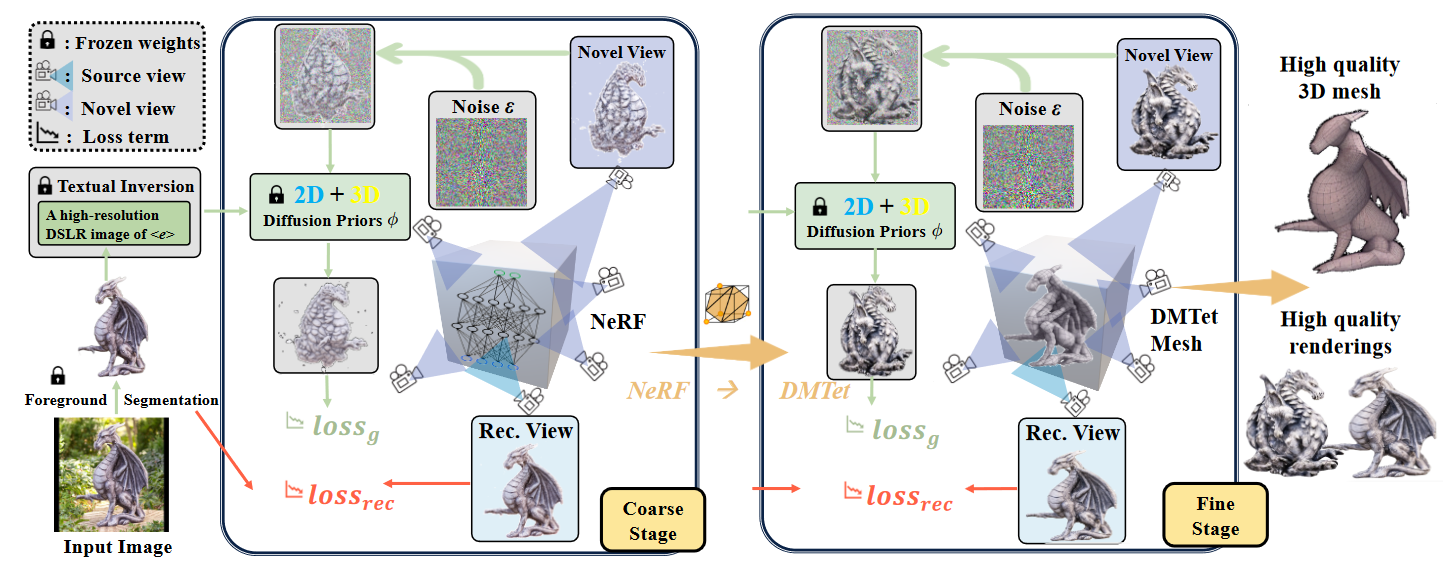
\includegraphics[width=1\columnwidth]{figures/Magic123.png}
      \caption{Summatized functionality of Magic123}\label{fig:figureMagic123}
\end{figure}
\subsection{Wonder 3D}\label{Wonder3D}

The primary innovation of Wonder3D lies in its ability to efficiently generate high-fidelity textured meshes from single images, a task that presents considerable challenges in the field of computer vision.

The method begins by generating consistent multi-view normal maps alongside corresponding color images through a cross-domain diffusion model. This process is critical for ensuring the fidelity and consistency of the generated 3D models. To achieve this, Wonder3D employs a multi-view cross-domain attention mechanism, which facilitates the exchange of information across different views and modalities, thereby enhancing the consistency and quality of the generated images \citep{long2023wonder3d}.

\begin{figure}[ht]
  \centering
    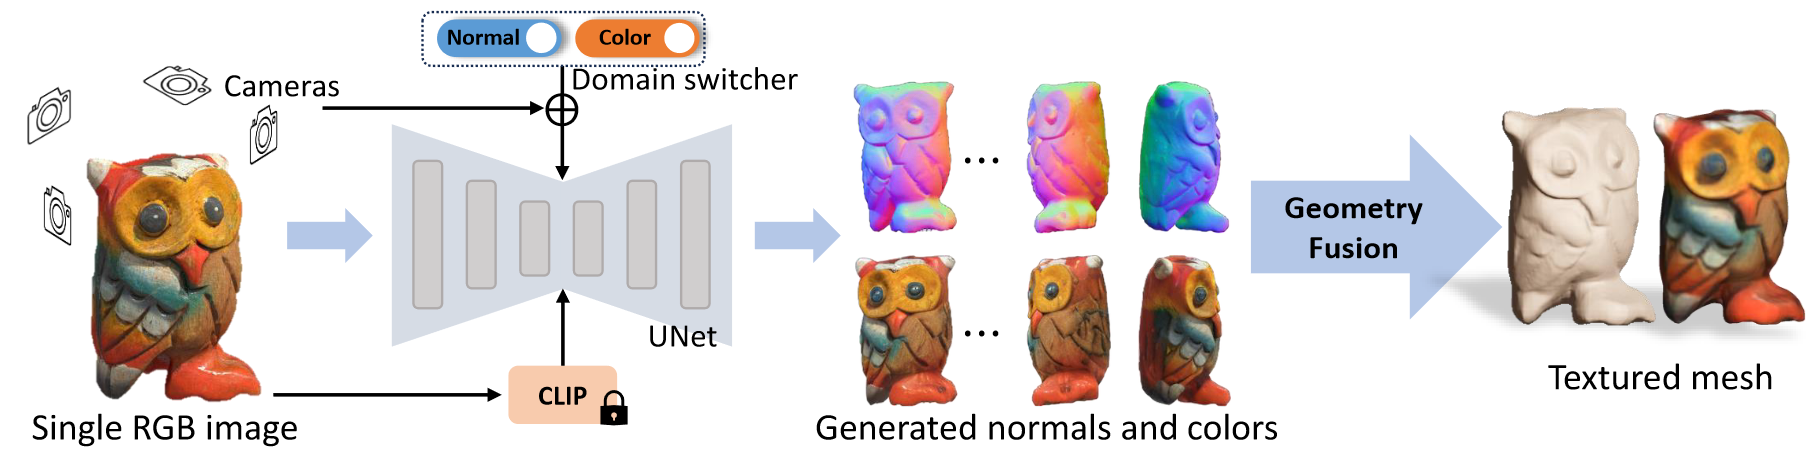
\includegraphics[width=1\columnwidth]{figures/Wonder3D.png}
    \caption{Summarized functionality of Wonder3D, depicting the method's unique approach to generating high-fidelity textured meshes from single images using cross-domain diffusion models \citep{long2023wonder3d}.}\label{fig:Wonder3D}
\end{figure}

An integral part of Wonder3D is its novel geometry-aware normal fusion algorithm. This algorithm robustly extracts high-quality surfaces from the generated multi-view 2D representations, including normal maps and color images. The fusion algorithm plays a pivotal role in reconstructing clean and detailed geometries from these 2D inputs, which is a significant step forward in the field \citep{long2023wonder3d}.

To understand this in simpler terms, imagine you have a single photo of an object, and you want to create a detailed 3D model of it. Traditional methods might struggle with this task, especially in terms of generating a model that is consistent and detailed from all angles. Wonder3D addresses this challenge by first creating multiple views of the object, as if you were looking at it from different angles. It does this by generating normal maps, which are like detailed blueprints of the object's surface textures and contours, as well as color images that match these maps. Then, using its specialized fusion algorithm, Wonder3D combines all these different views into a single, cohesive 3D model. This model not only looks good from the original angle of the photo but also from other angles, making it a more complete and accurate representation of the object.
